\documentclass[tikz,border=5pt]{standalone}
% Shared visual grammar: role fills, dark connectors, and 7-point typography.
% Build each standalone figure from this directory. No external images required.
\pdfinfoomitdate=1
\pdftrailerid{}
\usepackage[T1]{fontenc}
\usepackage{helvet}
\renewcommand{\familydefault}{\sfdefault}
\usepackage{amsmath,amssymb}
\hyphenpenalty=10000
\exhyphenpenalty=10000
\usetikzlibrary{arrows.meta,calc,fit,positioning,decorations.pathreplacing,backgrounds}
\definecolor{ink}{HTML}{172B3A}
\definecolor{muted}{HTML}{586D85}
\definecolor{datafill}{HTML}{F1F5F9}
\definecolor{dataline}{HTML}{62748E}
\definecolor{modelfill}{HTML}{E5E9FF}
\definecolor{modelline}{HTML}{7887C7}
\definecolor{llmfill}{HTML}{FFE4E8}
\definecolor{llmline}{HTML}{E68494}
\definecolor{truthfill}{HTML}{D0FAE5}
\definecolor{truthline}{HTML}{35A782}
\newcommand{\seven}{\fontsize{7}{8.5}\selectfont}
\tikzset{
 every node/.append style={font=\seven,text=ink,align=center},
 box/.style={draw=dataline,fill=white,rounded corners=3pt,line width=.65pt,inner sep=5pt,minimum height=8mm},
 data/.style={box,fill=datafill},
 model/.style={box,draw=modelline,fill=modelfill},
 llm/.style={box,draw=llmline,fill=llmfill},
 truth/.style={box,draw=truthline,fill=truthfill},
 title/.style={font=\seven\bfseries,inner sep=1pt},
 word/.style={text=muted,inner sep=1pt,align=center},
 label/.style={fill=white,inner xsep=2pt,inner ysep=1pt,text=muted},
 flow/.style={-{Stealth[length=2.4mm,width=1.9mm]},draw=ink,line width=1.2pt,shorten >=1.5pt},
 branch/.style={-{Stealth[length=2mm,width=1.6mm]},draw=ink,line width=.9pt,shorten >=1pt},
 route/.style={draw=ink,line width=1.2pt},
 update/.style={-{Stealth[length=2.2mm,width=1.7mm]},draw=modelline,line width=1pt,dash pattern=on 3pt off 2pt,shorten >=1.5pt},
 boundary/.style={draw=dataline,dash pattern=on 3pt off 2pt,rounded corners=3pt,line width=.6pt},
 chip/.style={minimum height=4mm,inner xsep=3pt,inner ysep=1.5pt,rounded corners=2pt},
}
% Optional role key. Anchor at the center of an uncluttered final row.
\newcommand{\rolekey}[2]{
 \node[word,anchor=east] at (#1-6.6,#2) {\textit{Key}};
 \node[data,chip] at (#1-5.2,#2) {records / data};
 \node[model,chip] at (#1-1.9,#2) {learned model / policy};
 \node[llm,chip] at (#1+1.65,#2) {LLM signal};
 \node[truth,chip] at (#1+4.95,#2) {labels / evaluation};
}

\newcommand{\emfont}{\fontsize{9}{11}\selectfont}
\begin{document}
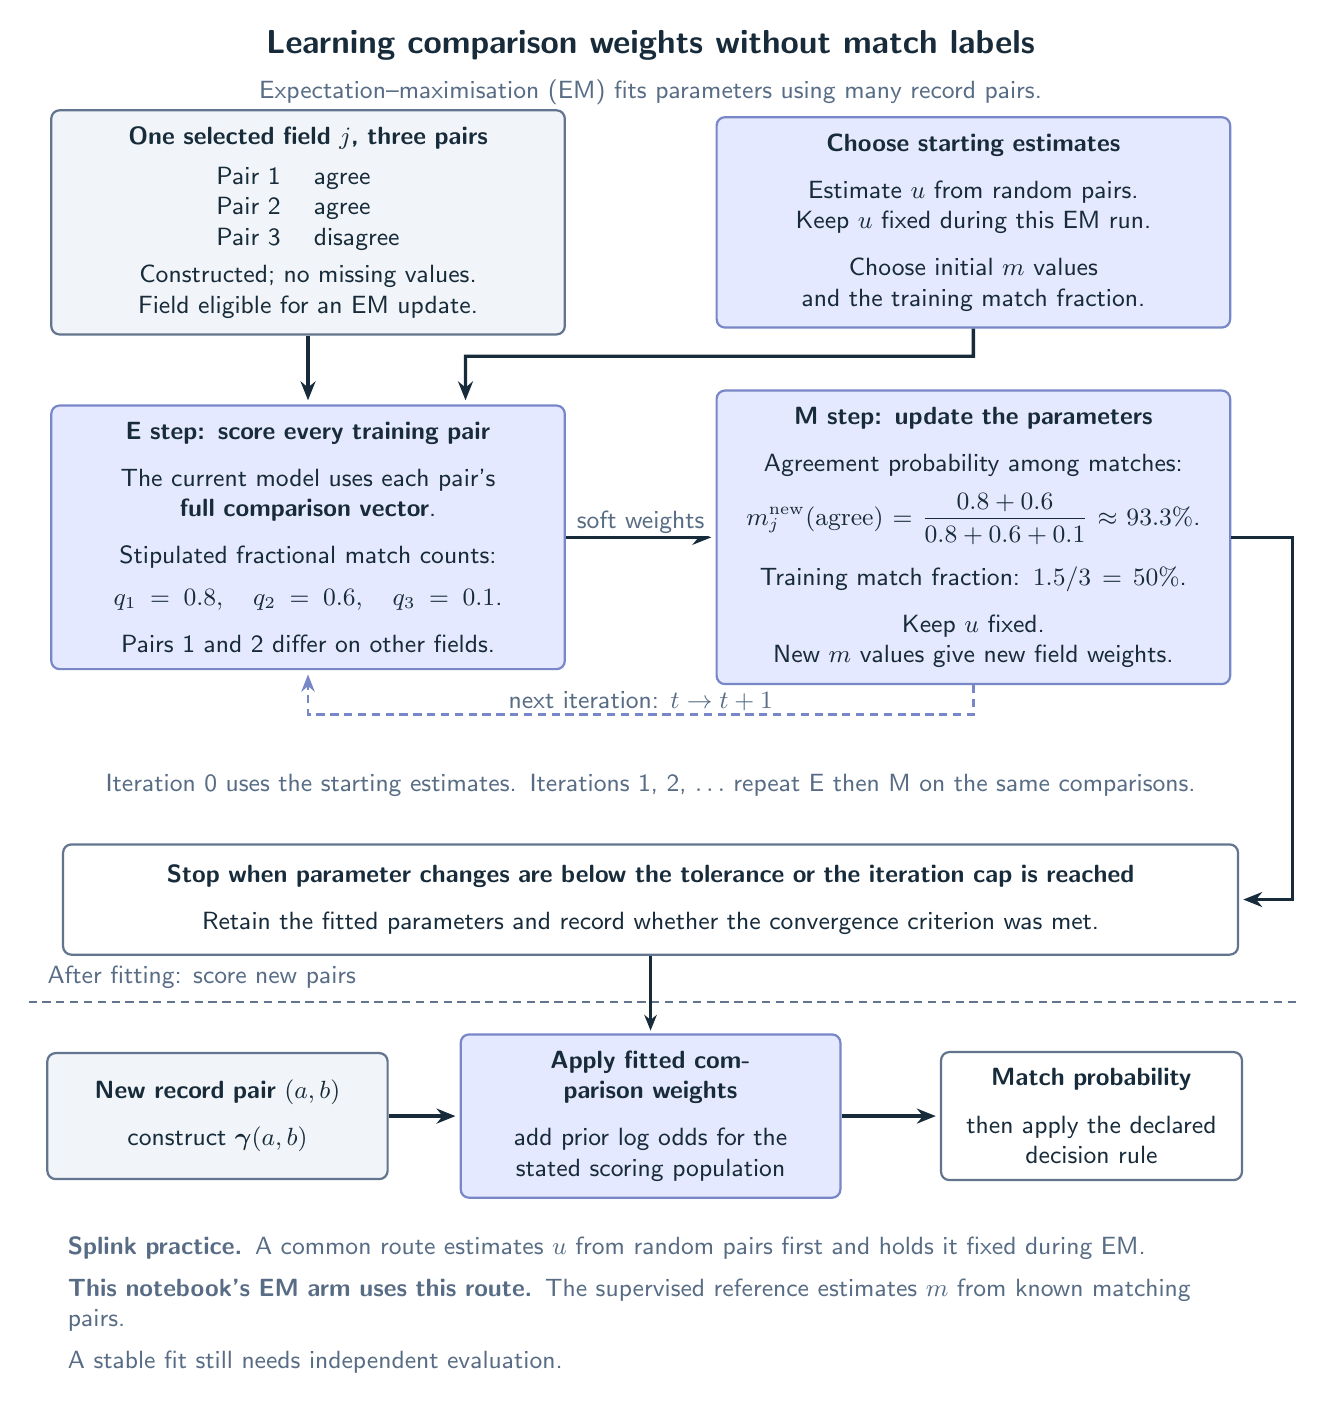
\begin{tikzpicture}[every node/.append style={font=\emfont},
  box/.append style={inner sep=6pt,line width=.8pt}]

\node[title,font=\fontsize{12}{14}\selectfont\bfseries] at (8,0) {Learning comparison weights without match labels};
\node[word] at (8,-.6) {Expectation--maximisation (EM) fits parameters using many record pairs.};

\node[data,text width=61mm,minimum height=20mm] (pairs) at (3.65,-2.25) {
  \textbf{One selected field $j$, three pairs}\\[4pt]
  \begin{tabular}{ll}
    Pair 1 & agree\\
    Pair 2 & agree\\
    Pair 3 & disagree
  \end{tabular}\\[3pt]
  Constructed; no missing values.\\
  Field eligible for an EM update.};
\node[model,text width=61mm,minimum height=20mm] (initial) at (12.1,-2.25) {
  \textbf{Choose starting estimates}\\[6pt]
  Estimate $u$ from random pairs.\\
  Keep $u$ fixed during this EM run.\\[6pt]
  Choose initial $m$ values\\
  and the training match fraction.};

\node[model,text width=61mm,minimum height=27mm] (expect) at (3.65,-6.25) {
  \textbf{E step: score every training pair}\\[6pt]
  The current model uses each pair's\\
  \textbf{full comparison vector}.\\[6pt]
  Stipulated fractional match counts:\\[4pt]
  $q_1=0.8,\quad q_2=0.6,\quad q_3=0.1$.\\[6pt]
  Pairs 1 and 2 differ on other fields.};
\node[model,text width=61mm,minimum height=27mm] (maximize) at (12.1,-6.25) {
  \textbf{M step: update the parameters}\\[6pt]
  Agreement probability among matches:\\[5pt]
  $m_j^{\mathrm{new}}(\mathrm{agree})=\dfrac{0.8+0.6}{0.8+0.6+0.1}\approx93.3\%$.\\[7pt]
  Training match fraction: $1.5/3=50\%$.\\[6pt]
  Keep $u$ fixed.\\
  New $m$ values give new field weights.};
\draw[flow] (pairs) -- (expect);
\draw[flow] (initial.south) -- (12.1,-3.95) -- (5.65,-3.95) -- ([xshift=20mm]expect.north);
\draw[flow] (expect) -- node[label,above] {soft weights} (maximize);
\draw[update] (maximize.south) -- (12.1,-8.5) -- node[label,above] {next iteration: $t\rightarrow t+1$} (3.65,-8.5) -- (expect.south);

\node[word,text width=145mm] at (8,-9.4) {Iteration 0 uses the starting estimates. Iterations 1, 2, $\ldots$ repeat E then M on the same comparisons.};
\node[box,text width=145mm,minimum height=14mm] (stop) at (8,-10.85) {
  \textbf{Stop when parameter changes are below the tolerance or the iteration cap is reached}\\[6pt]
  Retain the fitted parameters and record whether the convergence criterion was met.};
\draw[flow] (maximize.east) -- (16.15,-6.25) -- (16.15,-10.85) -- (stop.east);

\draw[boundary] (.1,-12.15) -- (16.2,-12.15);
\node[word,anchor=west] at (.3,-11.84) {After fitting: score new pairs};
\node[data,text width=39mm,minimum height=16mm] (newpair) at (2.5,-13.6) {
  \textbf{New record pair $(a,b)$}\\[6pt]
  construct $\boldsymbol\gamma(a,b)$};
\node[model,text width=44mm,minimum height=16mm] (fitted) at (8,-13.6) {
  \textbf{Apply fitted comparison weights}\\[6pt]
  add prior log odds for the\\
  stated scoring population};
\node[box,text width=34mm,minimum height=16mm] (result) at (13.6,-13.6) {
  \textbf{Match probability}\\[6pt]
  then apply the declared\\
  decision rule};
\draw[flow] (newpair) -- (fitted);
\draw[flow] (fitted) -- (result);
\draw[branch] (stop.south) -- (fitted.north);

\node[word,text width=148mm,align=left] at (8,-16.0) {
  \textbf{Splink practice.} A common route estimates $u$ from random pairs first and holds it fixed during EM.\\[4pt]
  \textbf{This notebook's EM arm uses this route.} The supervised reference estimates $m$ from known matching pairs.\\[4pt]
  A stable fit still needs independent evaluation.};

\end{tikzpicture}
\end{document}
